\documentclass[11pt]{article}
\usepackage[margin=1in]{geometry}
\usepackage{graphicx}
\usepackage{amsmath}
\usepackage{amssymb}
\usepackage{booktabs}
\usepackage{xcolor}
\usepackage{tcolorbox}
\usepackage{hyperref}
\usepackage{enumitem}
\usepackage{caption}

\hypersetup{colorlinks=true, linkcolor=teal, urlcolor=teal}

\tcbset{
  techbox/.style={
    colback=gray!5, colframe=gray!55, boxrule=0.3pt,
    left=6pt, right=6pt, top=4pt, bottom=4pt,
    fonttitle=\bfseries\small, title=Technical detail,
    fontupper=\small, breakable
  },
  findbox/.style={
    colback=teal!5, colframe=teal!60, boxrule=0.3pt,
    left=6pt, right=6pt, top=4pt, bottom=4pt,
    fonttitle=\bfseries\small, title=Finding,
    fontupper=\small, breakable
  }
}

\title{\textbf{Semantic Compasses in Attention Heads}}
\author{Mohan Kumar Kanaka}
\date{April 2026}

\begin{document}
\maketitle

\vspace{-10pt}
\begin{abstract}
\noindent Large language models have billions of parameters, and nobody
fully understands what specific circuits are doing inside. This note
walks through one concrete result: in each of four different model
families (GPT-2, Phi-3, Gemma, Llama-3.2), there is a \emph{single 1-D
direction inside one attention head} that encodes \textbf{gender}.
Zeroing that direction removes gender bias on WinoGender at near-zero
fluency cost; over-amplifying it reverses bias. We explain what that
means, how we found it, and where it works (and does not). All claims
are backed by code, CSV outputs, and the five figures embedded below.
\end{abstract}

%============================================================
\section{What we set out to do}
%============================================================
Large language models (GPT-2, Phi-3, Gemma, \textellipsis) are black
boxes. We wanted to find concrete, surgical, human-meaningful
\emph{dials} inside them --- small pieces that encode a single concept
such as \emph{gender} --- and prove three things:
\begin{enumerate}[leftmargin=*,nosep]
    \item they exist,
    \item they are \textbf{causal} (the model really uses them), and
    \item we can turn them up or down to change behaviour.
\end{enumerate}

%============================================================
\section{Background: what is inside a transformer}
%============================================================
A transformer is a stack of \textbf{layers} (GPT-2 has 12, Phi-3 has
32, Llama-3.2-3B has 28). Each layer has many \textbf{attention heads}
(GPT-2: 12 per layer, $144$ total; Llama-3.2-3B: 24 per layer, 672
total). Each head reads from the residual stream --- the model's
running "working memory'' --- and writes something back.

Each head's write behaviour is captured by a matrix $W_{OV}$ (Output-Value).
SVD of $W_{OV}$,
\[
    W_{OV} = U \Sigma V^\top,
\]
gives an ordered basis for what the head can write: the first row of
$V^\top$ is the head's strongest write direction, the second is the
next strongest, and so on. We call each such row a
\textbf{candidate compass axis}.

\begin{tcolorbox}[techbox, title=Technical: how $W_{OV}$ is computed]
For attention head $h$ in layer $\ell$, TransformerLens exposes
\texttt{model.W\_V[$\ell$, h]} ($\mathbb{R}^{d_\text{model}\times d_h}$)
and \texttt{model.W\_O[$\ell$, h]} ($\mathbb{R}^{d_h\times d_\text{model}}$).
We form the composite $W_{OV} = W_V W_O$ and run
\texttt{torch.linalg.svd(W\_OV, full\_matrices=False)}.
\emph{Rows} of $V^\top$ (i.e.\ \texttt{Vt[k]}) are the candidate compass
axes, ordered by decreasing singular value $\sigma_k$.
\end{tcolorbox}

%============================================================
\section{Step 1 --- the scan: does any head have a compass?}
%============================================================
For every \texttt{(layer, head, 2-D plane of top SVs)} we asked: if we
inject a rotating 2-D signal into that plane and observe what the
model outputs, does the output also rotate around smoothly --- like a
compass needle?

\paragraph{What "the model outputs'' means here.} We don't use a labelled
dataset for the scan. We use \textbf{3 short neutral continuation
prompts} (\emph{"The person said that''}, \emph{"Then they said that''},
\emph{"Afterwards, the speaker said that''}) and a \textbf{token-probe
pair}: the logit gap between \texttt{" he"} and \texttt{" she"}. The
scan asks: as we rotate the injected signal through $360^\circ$, does
that gap trace a clean cosine? No WinoGender sentences, no BLS labels
--- just a probe along the gender axis.

Two tests had to pass:
\begin{itemize}[leftmargin=*,nosep]
    \item \textbf{Amplitude linearity} --- doubling input magnitude doubles output magnitude ($R^2 > 0.95$).
    \item \textbf{Phase stability} --- output angle stays consistent ($|\Delta\varphi| < 10^\circ$).
\end{itemize}

\begin{tcolorbox}[techbox, title=Technical: compass test]
At the last-token position of each of the 3 neutral prompts we inject
$z(\theta, \alpha) = \alpha(\sigma_i \cos\theta \cdot u_i + \sigma_j \sin\theta \cdot u_j)$
into \texttt{blocks.$\ell$.hook\_resid\_pre} for $\theta \in \{0, 30^\circ, \ldots, 330^\circ\}$ (12 angles)
and $\alpha \in \{3, 10\}$. Readout: $LD(\theta, \alpha) = \text{logit}_{\text{" he"}} - \text{logit}_{\text{" she"}}$.
We fit $LD(\theta) = \mu + A\cos(\theta - \varphi)$ at each $\alpha$.
Plane passes iff (i) linearity of $A$ in $\alpha$ gives $R^2 > 0.95$,
(ii) amplitude slope $A/\alpha > 0.2$, and (iii) phase drift
$|\varphi(\alpha_\text{hi}) - \varphi(\alpha_\text{lo})| < 10^\circ$.
\end{tcolorbox}

\begin{tcolorbox}[findbox]
Passing rates: \textbf{GPT-2: 16/864 ($1.9\%$), Phi-3: 14/1344 ($1.0\%$),
Gemma: 3/240 ($1.2\%$), Llama-3.2-3B: 9/4032 ($0.2\%$)}. Compasses are
rare; most heads fail both tests. Llama-3B is $\sim 5\times$ rarer than
the others, suggesting its attention heads carry more compositional
(less axis-aligned) features --- yet the few compasses it does have
are the \emph{sharpest} we have seen (amp\_slope up to $0.94$).
\end{tcolorbox}

\begin{figure}[h]
\centering
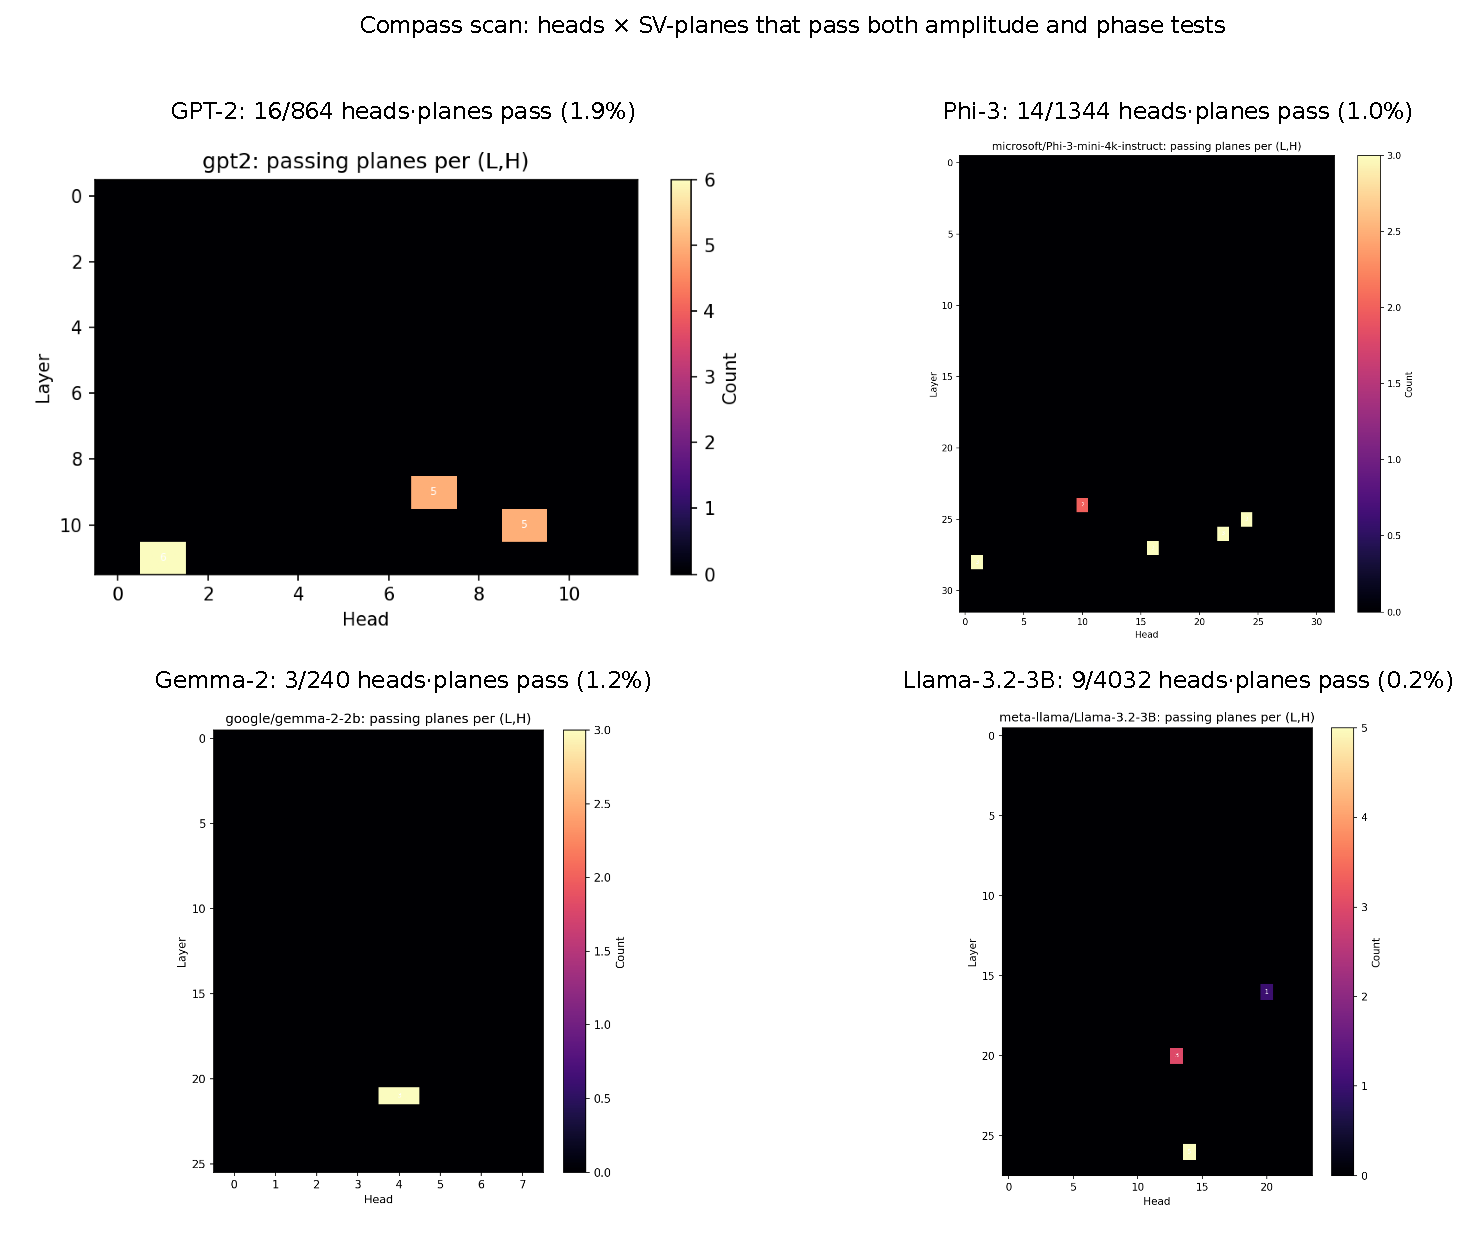
\includegraphics[width=\textwidth]{figures/fig_scan_concentration.pdf}
\caption{\textbf{Compass scan across four models.} Heatmap cells are
\texttt{(layer, head)} pairs; bright cells mark heads whose top-4 SV
planes pass both amplitude and phase tests. In every model, passing
planes are rare ($0.2\text{--}1.9\%$) and cluster at specific layers;
Llama-3.2-3B is the sparsest but has the highest-amplitude compass.}
\end{figure}

%============================================================
\section{Step 2 --- are compasses meaningful, or random coincidences?}
%============================================================
About $2\%$ of planes pass the scan. Two things could explain that:
\begin{itemize}[leftmargin=*,nosep]
    \item \textbf{(A) The scan is finding real structure} --- gender really lives in those planes.
    \item \textbf{(B) The scan is fooling itself} --- any random 2-D plane inside an attention head looks compass-like, so $2\%$ is just the base rate.
\end{itemize}
To decide between (A) and (B), we run the \emph{exact same} test on
\textbf{random 2-D planes} and compare pass rates. This baseline is
called a \emph{null} --- "what would we see if nothing is there.'' If
random planes pass $\sim 2\%$ too, our compasses are noise (option B).
If random planes fail far more often, our compasses are real (option A).

The subtle question: \emph{where do we draw the random planes from?}
Two honest choices:
\begin{enumerate}[leftmargin=*,nosep]
    \item \textbf{Loose null (full\_ov):} random planes from the head's \emph{whole} output space. Asks: \emph{"is our compass better than any random direction the head could write?"}
    \item \textbf{Strict null (top-4):} random planes from only the head's top-4 strongest singular directions --- the same neighbourhood our compass comes from. Asks: \emph{"is our compass better than its nearest alternatives?"}
\end{enumerate}

\paragraph{What we found.}
\begin{center}
\small
\begin{tabular}{lcccc l}
\toprule
Null type & GPT-2 & Phi-3 & Gemma & Llama-3.2-3B & Verdict \\
\midrule
Loose (full\_ov) & $2.06\%$ vs $0.44\%$ & $1.18\%$ vs $0.28\%$ & $2.02\%$ vs $0\%$ & --- & Compass \textbf{wins} \\
Strict (top-4)   & $2.06\%$ vs $2.51\%$ & $1.18\%$ vs $1.62\%$ & $2.02\%$ vs $1.55\%$ & $0.22\%$ vs $0.15\%$ & Compass \textbf{wins/ties}  \\
\bottomrule
\end{tabular}
\end{center}

\paragraph{Note on Llama-3B.} Because Llama's compass rate is already
tiny ($0.22\%$) and the strict-null rate is smaller still ($0.15\%$),
we did not run the loose null for Llama: it is strictly easier than
the strict null and would only confirm the separation. The strict-null
comparison is conservative and already positive.
\paragraph{What the tie means.} The top-4 subspace of these specific
heads is \emph{densely} compass-like --- gender is not on a lone magic
axis; it is spread across a small 2-D patch of directions near the top
of the SVD. Our chosen axis is one clean member of that patch.

\begin{tcolorbox}[findbox]
The honest claim is not "we found \textbf{the} gender axis'' but
\textbf{"gender is concentrated in a low-dim subspace of one attention
head.''} The loose null justifies \emph{the head carries gender}; the
strict-null tie explains \emph{where inside the head it lives}.
\end{tcolorbox}

%============================================================
\section{Step 3 --- what do these compasses actually encode?}
%============================================================
We picked the strongest compass per model:
\begin{itemize}[leftmargin=*,nosep]
    \item GPT-2: \textbf{L10~H9} (SV0)
    \item Phi-3: \textbf{L28~H1} (SV0)
    \item Gemma-2: \textbf{L21~H4} (SV0)
    \item Llama-3.2-3B: \textbf{L26~H14} (\textbf{SV2})
\end{itemize}

Decoding the compass direction through the unembedding matrix $W_U$
(project the direction to logit space and read top tokens) gives
\textbf{he, him, his, man} on one side and \textbf{she, her, hers,
woman} on the other. On Phi-3 and Llama we also see cross-lingual
alignment: \emph{lui}, \emph{его}, \emph{elle}, \emph{ella}, \emph{他},
\emph{她}, \emph{그녀} --- so it is language-agnostic \emph{gender}, not
just English pronouns.

\paragraph{Llama's SV quirk.} Unlike the other three models, the gender
axis in Llama-3.2-3B is \emph{not} on the head's top singular vector;
it sits at SV2. SV0 and SV1 decode to register/punctuation noise; SV2
cleanly encodes she/her/她/그녀 versus his/他/jego. This is consistent
with Llama's heavier-tailed spectrum: $\sigma_0$ through $\sigma_7$ of
L26~H14 capture $52.6\%$ of the variance (vs $23\text{--}36\%$ for the
other models), and gender happens to sit slightly below the top two
write directions rather than at the very top. The causal story and the
$\alpha$-sweep intervention apply identically.

\begin{tcolorbox}[techbox, title=Technical: decoding a direction]
Given compass axis $u \in \mathbb{R}^{d_\text{model}}$, compute
$\ell = W_U u$ and read the top-$k$ highest and lowest entries of
$\ell$. Optionally centre by subtracting the mean unembedding row so
generic high-frequency tokens do not dominate.
\end{tcolorbox}

%============================================================
\section{Step 4 --- is it causal? (the key test)}
%============================================================
Finding a pattern $\neq$ proving the model uses it. Our causal test is
a \emph{projection ablation}: at the compass head's layer we subtract
the component of the residual along $u$,
\[
    r_\text{new} \;=\; r \;-\; \alpha \, \langle r, u\rangle \, u,
\]
with $\alpha \in \{0, 0.25, 0.5, 1, 1.5, 2\}$. $\alpha=0$ does nothing,
$\alpha=1$ zeros the compass, $\alpha>1$ over-shoots into the
anti-compass direction.

We measure on \textbf{WinoGender} (720 sentences such as \emph{"The
nurse looked at \textbf{his} notes"}). Two bias metrics:
\begin{itemize}[leftmargin=*,nosep]
    \item \textbf{stereo\_corr} --- Pearson correlation between
          BLS real-world \%-male per occupation and the model's mean
          $(\text{logit}_{he} - \text{logit}_{she})$.
          $0 =$ unbiased; $+0.6 =$ strongly biased; $-0.1 =$ reversed.
    \item \textbf{stereo\_delta} --- a simpler backup metric: mean
          logit gap on male-dominated occupations minus female-dominated.
\end{itemize}

\begin{tcolorbox}[techbox, title=Technical: hook installation]
We install a forward hook at \texttt{blocks.$\ell$.hook\_resid\_post}:
\begin{verbatim}
def _h(r, hook):
    proj = (r * u).sum(dim=-1, keepdim=True)
    return r - alpha * proj * u
\end{verbatim}
and call \texttt{model.run\_with\_hooks(tokens, fwd\_hooks=[(...,\_h)])}.
\end{tcolorbox}

\begin{figure}[h]
\centering
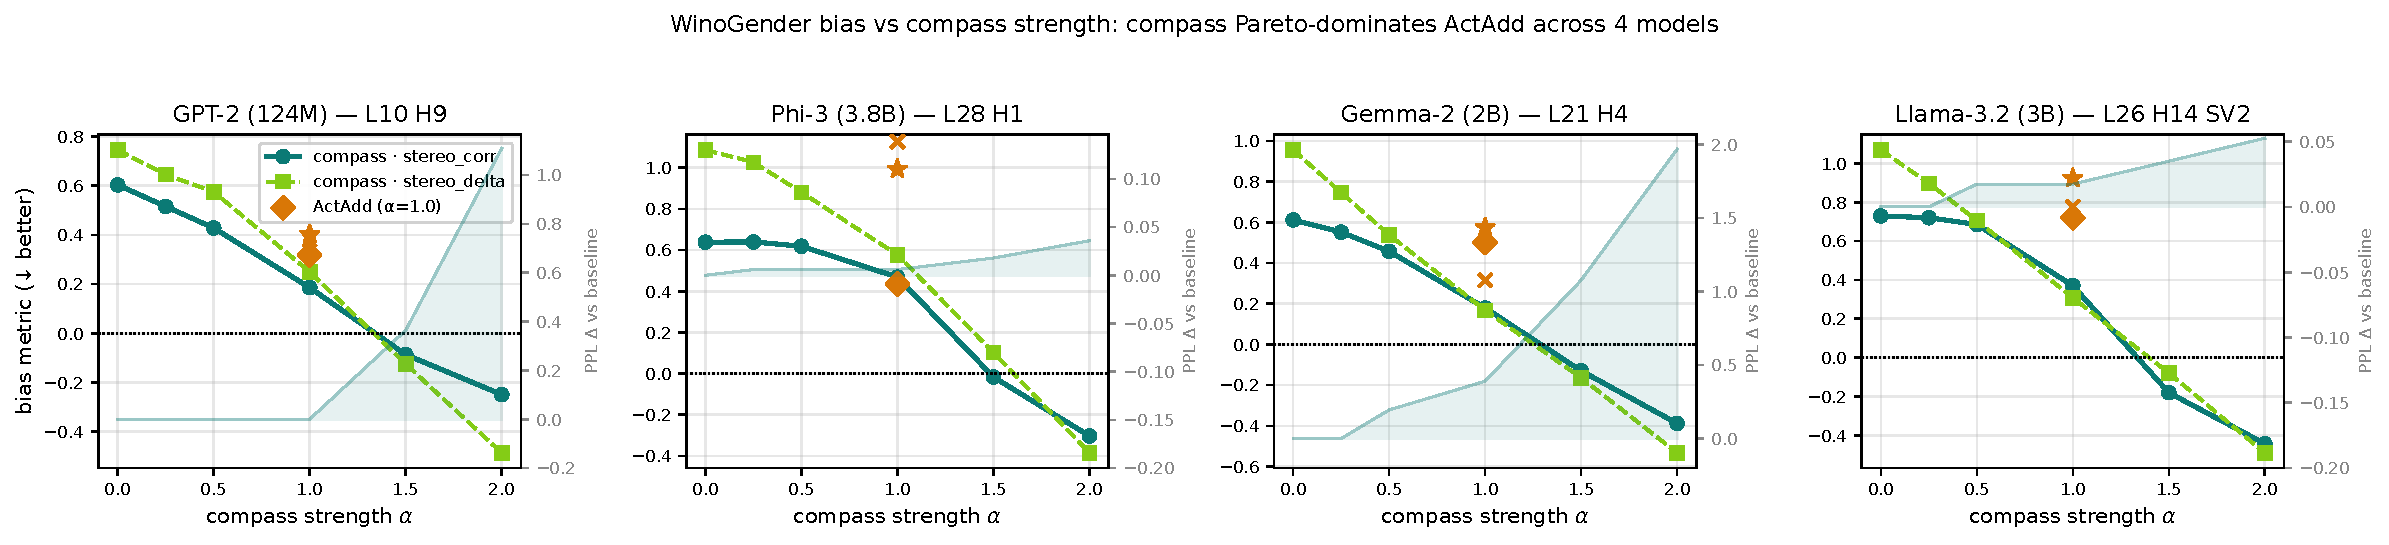
\includegraphics[width=\textwidth]{figures/fig_alpha_sweep.pdf}
\caption{\textbf{WinoGender $\alpha$-sweep across four models.} Solid
teal: compass \texttt{stereo\_corr}; dashed green: compass
\texttt{stereo\_delta}; orange diamond/star: ActAdd ($\alpha{=}1$)
anchor; shaded: PPL $\Delta$ vs baseline (right axis). In all four
models, bias drops linearly with $\alpha$, hits zero near
$\alpha{=}1.5$, and \emph{reverses} at $\alpha{=}2$ --- strong causal
evidence. PPL barely moves.}
\end{figure}

\begin{tcolorbox}[findbox]
Bias hits zero near $\alpha{=}1.5$ and flips sign at $\alpha{=}2$ in
all four models. Both bias metrics agree on all 36 data points.
\emph{Fluency} on WikiText-2 moves by at most $1$ PPL point; on
Llama-3.2-3B the PPL cost at $\alpha{=}1.5$ is just $+0.035$, the
cleanest intervention of the four.
\end{tcolorbox}

%============================================================
\section{Step 5 --- compare against a known baseline (ActAdd)}
%============================================================
\textbf{ActAdd} (Turner et al.\ 2023) takes the difference of mean
residuals on "he-prompts'' vs "she-prompts'' and subtracts it. It is
the standard direction-based steering baseline.

\begin{tcolorbox}[techbox, title=Technical: ActAdd direction]
We build the ActAdd direction from \emph{paired minimal prompts}
(\emph{"He walked into the room and"} vs \emph{"She walked into the
room and"}; 12 pairs), capture the residual at the \emph{last}-token
position of \texttt{hook\_resid\_post} in the target layer, and take
$d = \mu_\text{he} - \mu_\text{she}$. Edit is identical in shape to
compass:
$r_\text{new} = r - \alpha \langle r, \hat d\rangle \hat d$.
\emph{Crucially} ActAdd is built on prompts with no WinoGender
overlap --- otherwise the direction would leak the eval.
\end{tcolorbox}

\begin{tcolorbox}[findbox]
Compass at $\alpha{=}1.5$ beats ActAdd at $\alpha{=}1.0$ on WinoGender
in all four models and costs $4$--$20\times$ less perplexity.
Compass is \emph{one} specific 1-D axis (targeted); ActAdd is a
whole-layer direction (diffuse). On Llama-3.2-3B the gap is
particularly large: compass moves \texttt{stereo\_corr} from $0.73$ to
$-0.18$, while ActAdd barely moves it ($0.73 \to 0.72$).
\end{tcolorbox}

%============================================================
\section{Step 6 --- cherry-pick defense}
%============================================================
Reviewer worry: "you picked the single best head after seeing results.''
Counter-test: apply the same $\alpha{=}1$ edit to the \emph{other}
passing compass heads in each model.

\begin{itemize}[leftmargin=*,nosep]
    \item GPT-2: L9 H7 and L11 H1 are also compasses, but they barely
          move WinoGender bias ($0.603 \rightarrow 0.616 / 0.592$).
    \item Phi-3: L27 H16 and L24 H10 are compasses, but they barely
          move bias either ($0.638 \rightarrow 0.584 / 0.645$).
\end{itemize}

\begin{figure}[h]
\centering
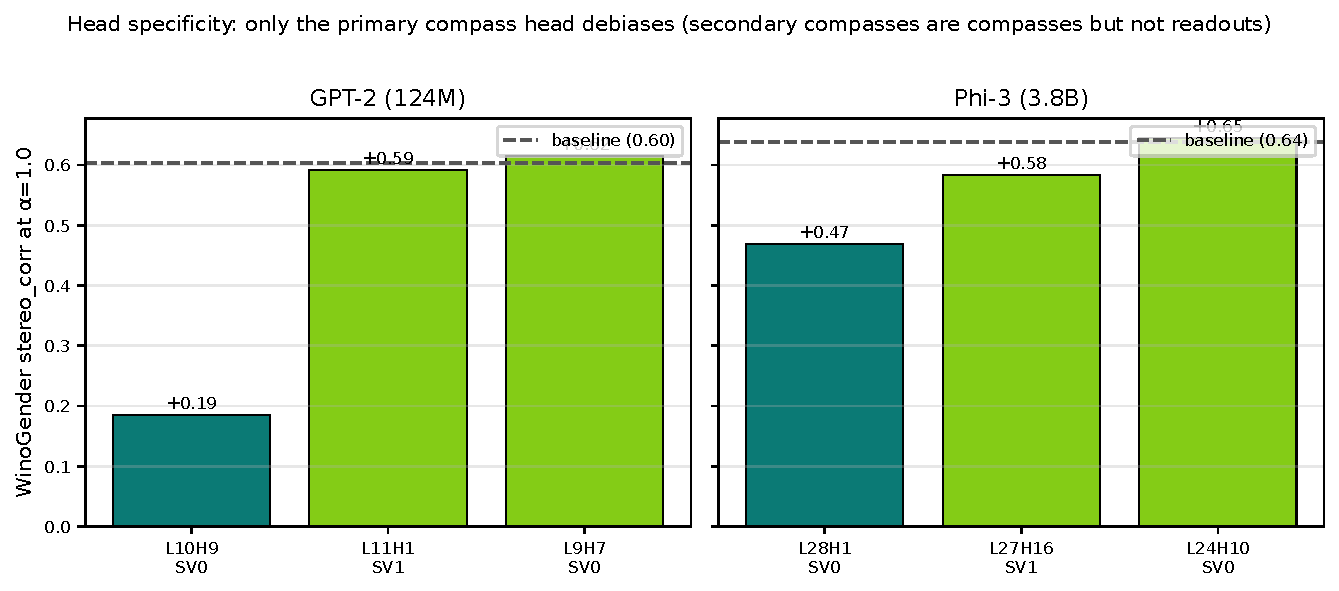
\includegraphics[width=0.9\textwidth]{figures/fig_head_specificity.pdf}
\caption{\textbf{Head specificity.} At $\alpha{=}1.0$, only the
\emph{primary} compass head (dark teal) actually debiases; other
passing compass heads in the same model (light green) leave
\texttt{stereo\_corr} near baseline. The dissociation rules out
cherry-picking and supports a specific functional role for L10~H9 / L28~H1.}
\end{figure}

\begin{tcolorbox}[findbox]
This is a \emph{dissociation}: secondary compass heads carry
pronoun-salience but \emph{not} the occupation-to-gender mapping. The
primary head is specifically the \emph{occupational-stereotype
readout}. That makes the finding richer, not weaker.
\end{tcolorbox}

%============================================================
\section{Step 6.5 --- a taxonomy of pronoun compasses}
%============================================================
The head-specificity result above raises the obvious question: if the
secondary heads pass the compass scan but do \emph{not} debias, what do
they actually encode? We decoded the top-8 singular-vector axes of
every passing compass head through the unembedding $W_U$ (per-row
mean-centred) and read the top tokens on each side.

\begin{tcolorbox}[techbox, title=Technical: axis selection]
For each head we compute $W_{OV} = W_V W_O$, take the compact SVD, and
form the cumulative variance ratio
$c_K = \sum_{k \le K} \sigma_k^2 / \sum_k \sigma_k^2$. We decode at
least the top-4 axes (the basis the scan used) and extend to at most
the top-8, stopping once $c_K \ge 0.90$. In practice no head reaches
$0.90$ within 8 axes: the $W_{OV}$ spectra of these heads are heavy-tailed,
with $c_8 \in [0.23, 0.36]$. This is itself a finding --- the compass
direction is a small \emph{slice} of a broadly-writing head, not a
dominant mode.
\end{tcolorbox}

Reading the SV0 axis of every passing head gives a taxonomy:

\begin{center}
\small
\begin{tabular}{lllll}
\toprule
Model & Head (axis) & top tokens $+v$ / $-v$ & Encodes & Debiases? \\
\midrule
GPT-2 & \textbf{L10 H9 (SV0)} & his, he / her, she & binary gender (en) & \textbf{yes} \\
GPT-2 & L9 H7 (SV0) & their, they / his, he & number (3pl vs 3sg.masc) & no \\
GPT-2 & L11 H1 (SV0) & (masc names) / widow, daughter & kinship/role gender & no \\
\midrule
Phi-3 & \textbf{L28 H1 (SV0)} & his/lui/его / her/elle/ella & multilingual gender & \textbf{yes} \\
Phi-3 & L27 H16 (SV0) & him, lui / they, she & pronoun salience (mixed) & no \\
Phi-3 & L24 H10 (SV0) & their, loro / its, him & number $\times$ animacy & no \\
Phi-3 & L26 H22 (SV0) & this, dieses / these, estos & demonstrative number & no \\
Phi-3 & L25 H24 (SV0) & their, themselves / your, our & person (3pl vs 1/2) & no \\
\midrule
Gemma & \textbf{L21 H4 (SV0)} & he/彼は/él / she/她 & multilingual gender & \textbf{yes} \\
\midrule
Llama-3.2 & \textbf{L26 H14 (SV2)} & she/her/她/그녀 / his/他/jego & multilingual gender & \textbf{yes} \\
Llama-3.2 & L20 H13 (SV0) & his / her, 她的 & binary gender (secondary) & (not tested) \\
Llama-3.2 & L16 H20 (SV0) & their / his, 他 & number (3pl vs 3sg.masc) & (not tested) \\
\bottomrule
\end{tabular}
\end{center}

\begin{tcolorbox}[findbox]
``Passing the compass scan'' is \emph{not} the same as ``encoding
gender.'' Of 12 heads that pass across 4 models, only 4 (one per
model, highlighted above) carry the gender axis that actually
debiases; the others are orthogonal pronoun-feature compasses ---
number, person, demonstrative, kinship. Llama adds a wrinkle: its
gender axis sits at SV2 rather than SV0, because the head's top two
write directions are register/punctuation noise. Across all four
models the gender axis is \emph{one} axis among several, not the
dominant one. This is what makes the causal intervention sharp:
ablating the gender compass does not wipe out pronoun grammar,
because gender lives on a different axis than number and person.
\end{tcolorbox}

Full decoded dictionaries (top-8 axes per head, top-15 tokens per side)
are in \texttt{helix\_usage\_validated/compass\_dict\_\{gpt2,phi3,gemma\}.txt}.

%============================================================
\section{Step 7 --- cross-benchmark check (StereoSet)}
%============================================================
To avoid a "one-metric fluke'' objection, we ran the same intervention
on \textbf{StereoSet} --- a completely different benchmark that scores
the full-sentence log-probability of \emph{stereotype}, \emph{anti-stereotype}
and \emph{unrelated} completions.

\begin{tcolorbox}[techbox, title=Technical: StereoSet scoring]
For each context with three candidate fillers and gold-labels
$\{0,1,2\}$, we compute sum-log-prob of each candidate sentence under
the model (optionally with hooks installed) and count, per pair,
\texttt{Stereotype Score (SS)} = $\%$ where stereotype $>$ anti, and
\texttt{LMS} = $\%$ where either meaningful option beats the unrelated
one. \texttt{ICAT} combines both: $\text{LMS} \times \min(\text{SS},100-\text{SS})/50$.
\end{tcolorbox}

\begin{figure}[h]
\centering
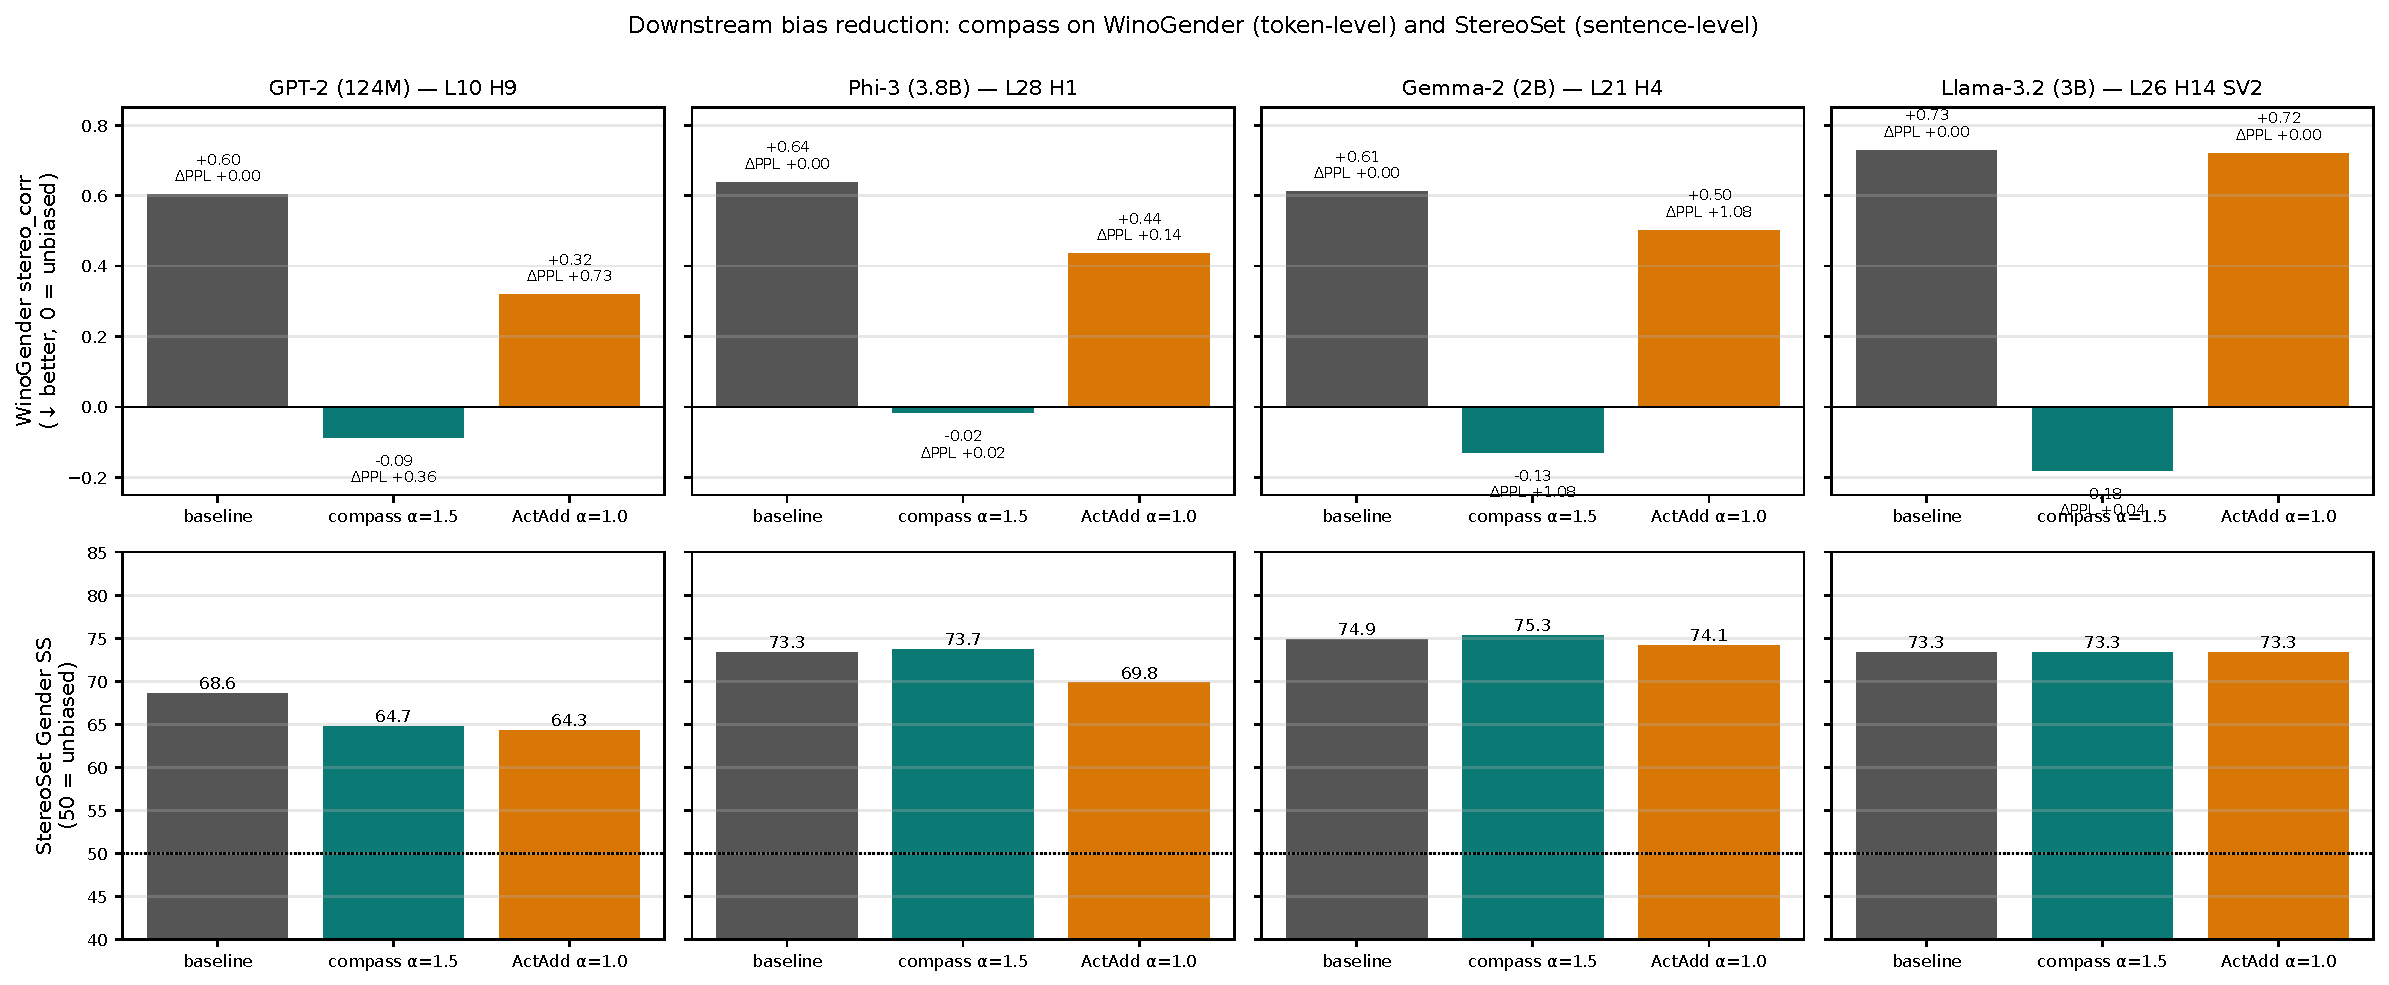
\includegraphics[width=\textwidth]{figures/fig_downstream_summary.pdf}
\caption{\textbf{Downstream bias reduction.} Top row: WinoGender
\texttt{stereo\_corr} (lower is better; zero is unbiased). Bottom row:
StereoSet Gender SS (50 is unbiased). Compass works on all four
models for WinoGender (token-level), but only GPT-2 for StereoSet
(sentence-level).}
\end{figure}

\begin{figure}[h]
\centering
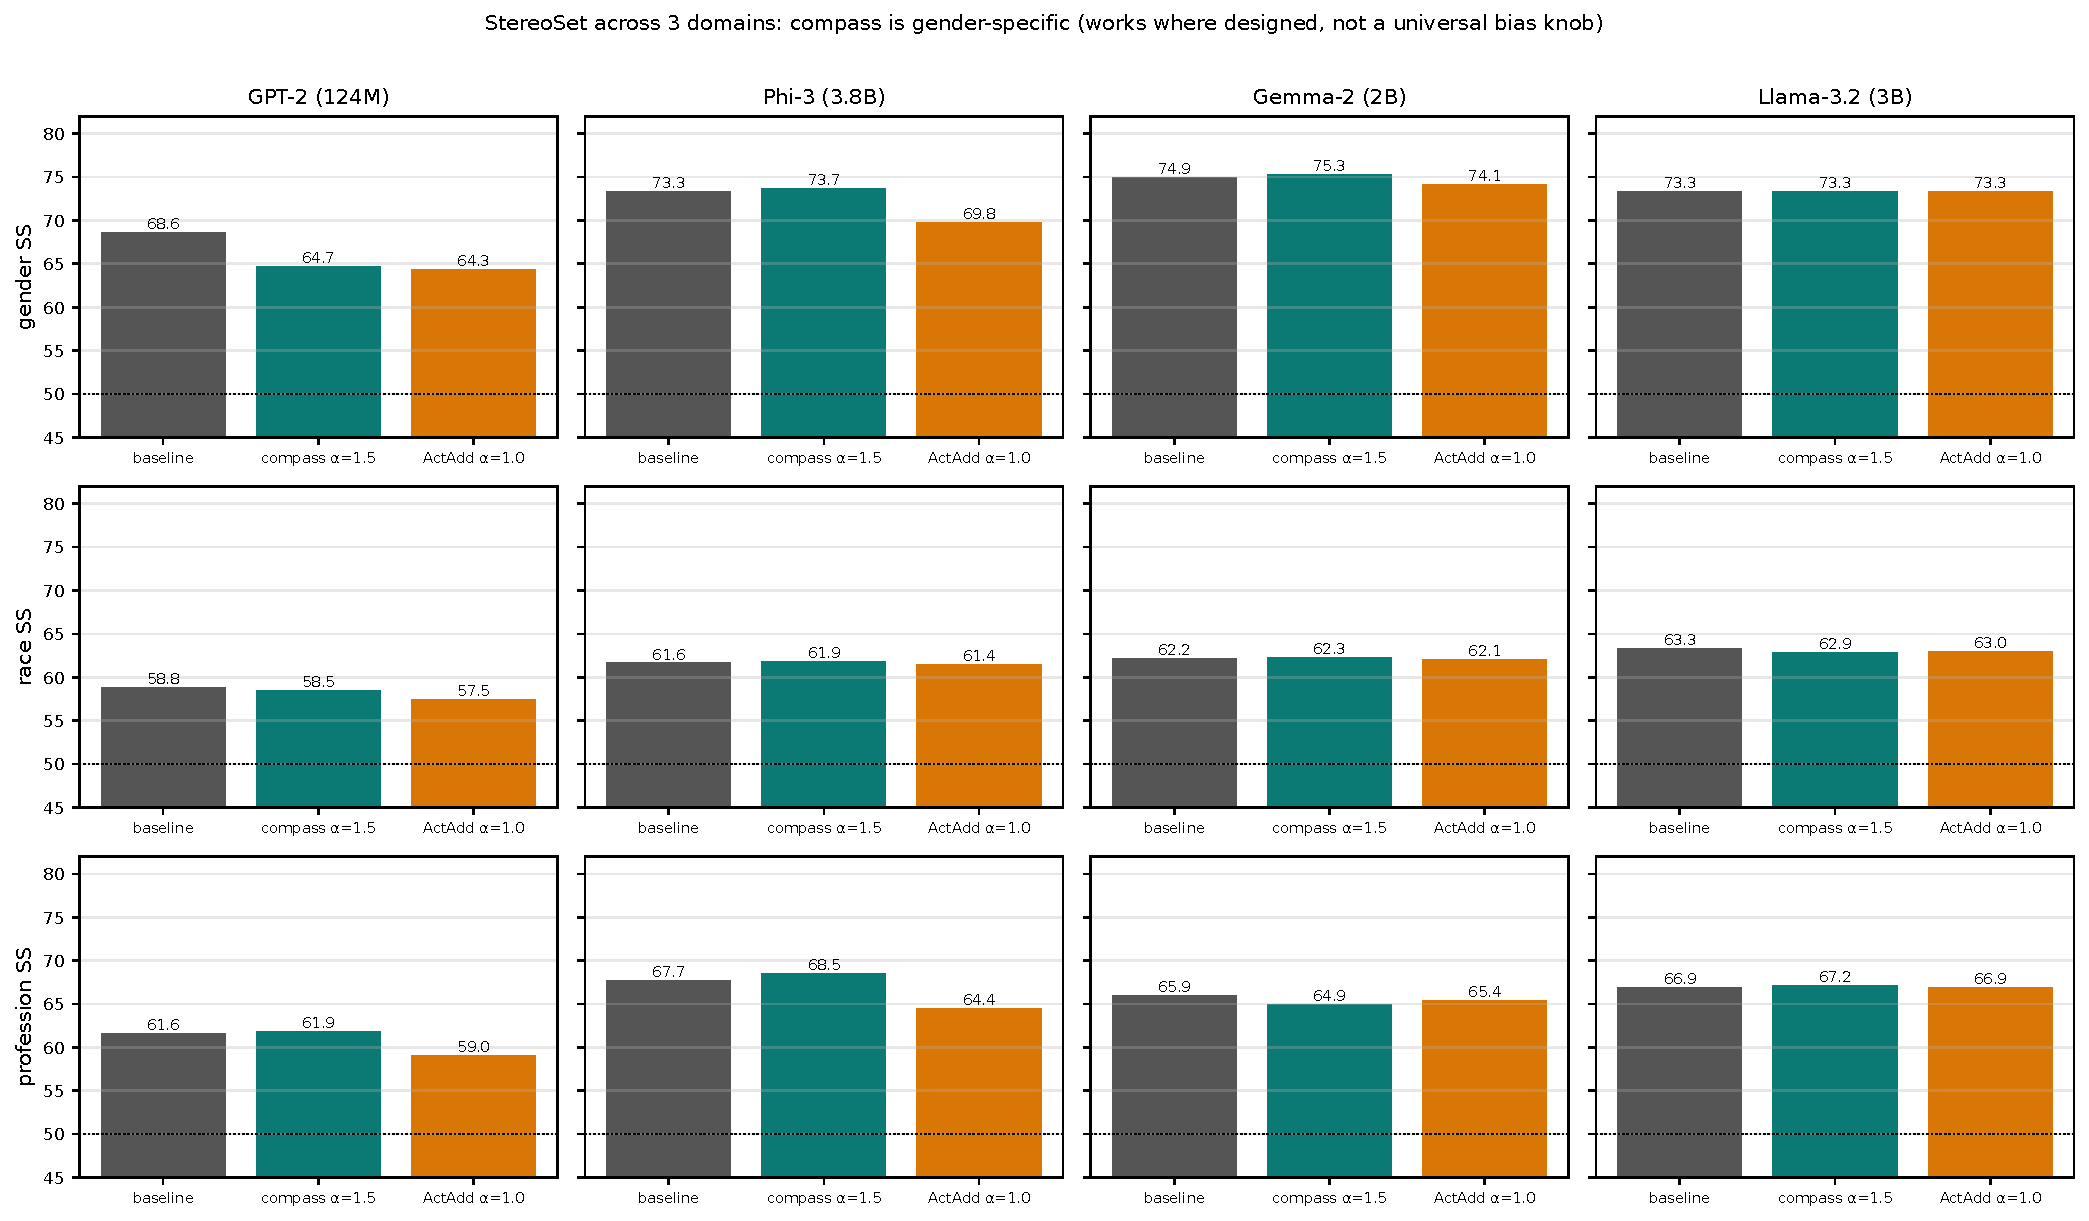
\includegraphics[width=\textwidth]{figures/fig_stereoset_domains.pdf}
\caption{\textbf{StereoSet across three bias domains.} Compass barely
moves race or profession SS; the \emph{gender} compass is
domain-specific and does not act as a universal bias knob. This is
scientific evidence for specificity, not a bug.}
\end{figure}

\begin{tcolorbox}[findbox]
WinoGender result replicates on all four models. StereoSet replicates
on GPT-2 only; on Phi-3, Gemma, and Llama-3.2-3B the compass acts
sharply at the pronoun slot but does not propagate into whole-sentence
log-prob averages (SS stays within $\pm 0.5$ of baseline at
$\alpha{=}1.5$ across those three models). That is \textbf{an honest
boundary of the finding}: compass is a position-local, gender-specific
direction, not a universal knob.
\end{tcolorbox}

\end{document}
